\chapter{TINJAUAN PUSTAKA}
\section{Penelitian Terdahulu}
\hspace{25pt}Penelitian yang berkaitan dengan identifikasi potensi panas bumi baik menggunakan metode penginderaan jauh landsat 8 maupun metode gravitasi telah beberapa kali dilakukan sebelumnya, contohnya seperti penelitian yang dilakukan oleh\citep{Rosyiful2019} dengan judul "Identifikasi Struktur Bawah Permukaan Daerah Prospek Panas Bumi dengan Metode Gravitasi".  Penelitian tersebut dilakukan di daerah mata air panas Padusan Mojokerto dengan pengukuran langsung di lapangan menggunakan gravimeter La Coste Romberg. Data lapangan yang diperoleh selanjutnya dilakukan konversi ke mGal dan kemudian dilakukan beberapa koreksi seperti koreksi tidal, drift, udara bebas, Bouguer hingga akhirnya diperoleh anomali Bouguer lengkap. Anomali Bouguer lengkap yang diperoleh masih dipengaruhi oleh ketinggian sehingga dilakukanlah reduksi ke bidang datar. Kemudian dilakukan pemisahan anomali untuk memperoleh anomali lokal dan regional serta dilakukan analisa spektrum untuk mengetahui kedalaman optimum dari anomali. Anomali regional memiliki jangkauan yang lebih dalam sedangkan anomali lokal atau residual memiliki kedalaman yang lebih dangkal atau lebih dekat dengan permukaan. Berdasarkan analisa spektrum diperoleh kedalaman anomali regional mencapai 1140 m sedangkan anomali lokal sebesar 127 m di bawah permukaan. Kemudian dari peta anomali lokal tersebut dilakukan analisis derivatif menggunakan filter \textit{First Horizontal Derivative} (FHD) dan \textit{Second Vertical Derivative }(SVD). Analisis derivatif ini dilakukan untuk mengetahui adanya patahan serta jenisnya. Selain analisis derivatif, peta anomali lokal digunakan untuk pemodelan 3D struktur bawah permukaan berdasarkan nilai densitas batuan. Diperoleh hasil bawah permukaan didominasi oleh andesit, tanah, lempung, lava basaltik dan \textit{eclogit}.

\hspace{25pt}Penelitian lainnya dilakukan oleh \citep{Faisal2019} dengan judul "Pemetaan Potensi Geothermal Seulawah Agam Berdasarkan Data DEMNAS dan Landsat 8". Lokasi penelitian berada di Gunung Seulawah Agam yang merupakan salah satu gunung api aktif di Aceh. Penelitian ini tentu menggunakan data sekunder dimana Landsat merupakan citra satelit program dari USGS dan \textit{Digital Elevation Model} Nasional (DEMNAS) merupakan peta elevasi program Badan Informasi Geospasial Indonesia. Data Landsat 8 terdiri dari 11 band dimana hanya digunakan 4 band saja yaitu band 3,4,5 dan 10. Band 4 dan 5 digunakan untuk analisis \textit{Normalized Differential Vegetation Index} (NDVI) yaitu untuk menghitung kerapatan vegetasi, Band 3 dan 5 untuk analisis \textit{Normalized Differential Water Index} (NDWI) yaitu untuk menghitung tingkat kebasahan suatu area dan band 10 adalah band thermal untuk mendeteksi suhu permukaan. Pengolahan data Landsat 8 dilakukan hingga diperoleh \textit{Land Surface Temperature} (LST) sehingga dapat diperoleh sebaran panas dipermukaan daerah penelitian. Data DEMNAS dilakukan konversi hingga diperoleh \textit{hillshade} yang selanjutnya dilakukan penarikan kelurusan untuk memperoleh \textit{Fault Fracture Density} (FFD) yaitu densitas sesar dan rekahan. Dari penelitian ini diperoleh sebaran potensi panas bumi dengan mengkorelasikan antara LST, NDVI, NDWI dan FFD bahwa lokasi yang berkaitan dengan potensi panas bumi memiliki FFD sedang ke tinggi dengan nilai 0.3 - 0.9 $km/km^2$ semudian NDVI dan NDWI menunjukkan vegetasi yang jarang dan LST yang tinggi pada manifestasi panas bumi.

\hspace{25pt}Kemudian penelitian yang menggabungkan kedua metode tersebut yaitu menggunakan data Landsat 8 dan metode gravitasi telah dilakukan oleh \citep{Wiyono2022} dengan judul \textit{"Gravity and Remote Sensing Methods as a Solution in Identifying Geothermal Reservoirs on Volcanoes"}. Lokasi penelitian ini adalah di Tiris, Gunung Lamongan Probolinggo. Dari segi pengambilan data, penelitian ini sama dengan dua penelitian di atas. Data gravitasi diperoleh melalui pengukuran langsung dilapangan dan data Landsat dari USGS. Sedikit perbedaan terdapat pada data DEM dimana pada penelitian ini yang digunakan adalah DEM SRTM \textit{(Shuttle Radar Topography Mission)}. Perbedaan lainnya adalah tidak dilakukannya analisis derivatif dan FFD. Hasil penelitian ini adalah ditemukan lapisan batuan reservoir dengan densitas $2.8 - 2.83g/cm^3$ dan kedalaman 500 - 800m yang termasuk kedalam batuan vulkanik dan breksi, lapisan batuan beku intrusif dengan densitas $2.84-2.86 g/cm^3$ dan kedalaman sekitar 350 m. Sebaran suhu permukaan pada daerah penelitian berkisar 15,84°C hingga 41,05°C, namun pada lokasi manifestasi panas bumi di Desa Tiris, tidak terlihat adanya anomali LST karena adanya percampuran antara suhu air panas panas bumi dan suhu aliran air Sungai Tancak.
\section{Geologi Penelitian}
\hspace{25pt}Gunung Lamongan adalah salah satu gunung api aktif di Jawa Timur. Gunung ini bertipe strato dengan ketinggian mencapai 1671 mdpl. Secara administratif, G.Lamongan berada di dua kabupaten yaitu Probolinggo dan Lumajang dengan koordinat di puncaknya adalah $7^{\circ}59'$LS dan $113^{\circ},5'$BT. G. Lamongan merupakan gunung api muda yang berasal dari pensesaran G. Tarub yang berada di sebelah timur. Pensesaran ini mengarah dari tenggara ke barat laut yang mengakibatkan bagian barat G. Tarub runtuh yang kemudian pada bagian ini tumbuh menjadi G. Lamongan. Berdasarkan data dari Badan Geologi Pusat Vulkanologi dan Mitigasi Bencana Geologi, G. Lamongan mengalami erupsi dengan periode yang variatif dalam interval tahun 1799 hingga 1898. Kemudian di tahun-tahun berikutnya terjadi gempa bumi tektonik lokal yang mengakibatkan terjadinya retakan tanah\citep{GLamongan}. 

\hspace{25pt} Gunung Lamongan memiliki karakteristik yang menarik daripada gunungapi lainnya di Jawa Timur. Di sekitar gunung ini terdapat sekitar 64 pusat erupsi parasit yang terdiri dari 37 kerucut vulkanik dan 27 buah “maar”. Beberapa kerucut vulkanik tersebut adalah kerucut G. Jalak, G. Pakem, dan G. Pakis. Kemudian terdapat maar yang berbentuk ranu dimana 13 ranu diantaranya terisi air seperti Ranu Klakah, Ranu Pakis, Ranu Bedali dan beberapa Ranu lainnya. Tetapi diantara 13 Ranu yang ada, juga dijumpai beberapa Ranu yang sudah tidak terisi air lagi. Kemungkinan disebabkan oleh penurunan muka air atau pola air tanah yang menyebar di sekitarnya \cite{GLamongan}. 

\hspace{25pt} Berdasarkan data geologi, produk dari Gunungapi Lamongan dapat dibagi menjadi beberapa kategori, seperti produk erupsi pusat G. Tarub (Lamongan Tua), Lamongan Muda (Lamongan Sekarang), hasil erupsi samping, erupsi eksentrik, erupsi freatik, dan endapan sekunder. Hasil erupsi kawah pusat terdiri dari lava dan jatuhan piroklastik, sedangkan hasil erupsi samping cenderung berupa aliran lava. Erupsi eksentrik, pada umumnya terdiri dari lava saja atau piroklastik dan kombinasi dari keduanya. Endapan sekunder umumnya berupa lahar dan endapan fluviatil. Namun, tidak ditemukan produk erupsi G. Lamongan yang berupa endapan aliran piroklastik baik dari data penelitian sebelumnya maupun hasil penyelidikan di lapangan. Dengan mengacu pada stratigrafi daerah Probolinggo dan Lumajang, maka stratigrafi regional daerah survey terdiri dari enam satuan. Masing-masing satuan mulai dari yang tertua sampai yang termuda adalah Satuan Batuan Gunungapi Tengger (Qvt), Satuan Tuf Argopuro (Qvat), Satuan Tuf Argopuro (Qvab), Satuan Gunungapi Lamongan (Qvl), dan Satuan Lava Lamongan (Qvll)\cite{GLamongan}.

\hspace{25pt} Di sisi timur G. Lamongan terdapat desa Segaran yang masuk dalam kecamatan Tiris. Di desa ini ditemukan dua mata air panas di lokasi yang berdekatan dengan suhu sekitar $42-46^{\circ}C$. Daerah panas bumi Tiris memiliki kontrol struktural regional dari arah barat laut ke tenggara dan utara ke selatan, yang merupakan arah struktur utama di pulau Jawa. Struktur-struktur ini juga mempengaruhi kemunculan mata air panas di sebelah timur laut. Data geokimia menunjukkan adanya indikasi reservoir bertemperatur tinggi pada kedalaman yang signifikan, yang berasal dari Gunung Lamongan. Terdapat potensi cadangan yang diperkirakan di sekitar Gunung Lamongan dan merentang ke arah barat daya selama sekitar $11 km^2$, dengan estimasi potensi sebesar 74 MWe dan luas wilayah sekitar $299 km^2$ atau sekitar 29.900 Ha \cite{GLamongan}.

\begin{figure}[h]
	\centering
	\includegraphics[scale=1.2]{Figs/geologi.jpg}
	\caption{Peta geologi Tiris-Gunung Lamongan}
	\label{fig:geologi}
\end{figure}

\section{Sistem Panas Bumi}
\hspace{25pt}Panas bumi atau geothermal adalah energi dalam bentuk fluida baik air atau uap panas yang tersimpan di batuan reservoir yang terdapat pada kerak bumi \citep{GuptaRoy2007}. Sistem panas bumi dibangun oleh beberapa komponen penting seperti sumber panas, fluida, batuan reservoir dan lapisan penudung. Sumber panas bumi berasal dari intrusi batuan, dapur magma atau gradien temperatur. Intrusi batuan dan dapur magma dapat ditemukan di daerah dekat gunungapi sedangkan gradien temperatur berada di daerah lempeng tektonik aktif atau cekungan sedimen. Sumber panas bumi berupa intrusi magmatik berada pada kedalaman sekitar 5-10km dengan suhu lebih dari $600^{\circ}C$ \citep{DicksonFanelli1995}. 

\hspace{25pt}Fluida panas bumi berupa air yang sering ditemukan berjenis meteorik dalam fase cair atau uap yang membawa senyawa karbondioksida, hidrogen sulfida, dan lainnya. Air meteorik merupakan air tanah yang berasal dari atmosfer bumi dalam bentuk hujan atau salju. Air ini kemudian masuk menuju bawah permukaan melalui pori batuan atau patahan yang kemudian tersimpan di batuan reservoir. Reservoir adalah batuan berpori dengan porositas dan permeabilitas yang baik. Porositas adalah persentase volume pori atau ruang kosong dalam batuan terhadap volume batuan dan permeabilitas adalah kemampuan batuan untuk meloloskan fluida. Pada zona inilah fluida akan tersimpan sehingga semakin tinggi porositas dan permeabilitasnya maka semakin banyak fluida yang ditampung. Reservoir ini kemudian akan mengalami pemanasan oleh sumber panas \citep{DicksonFanelli1995}.

\hspace{25pt}Batuan penudung yaitu batuan dengan permeabilitas rendah bertugas untuk mencegah fluida panas bumi keluar dari reservoir. Batuan penudung berada di atas reservoir kemudian batuan dasar dengan permeabilitas rendah berada di bawah reservoir untuk mencegah fluida panas bumi turun akibat gravitasi \citep{GuptaRoy2007}.


\begin{figure}[h]
	\centering
	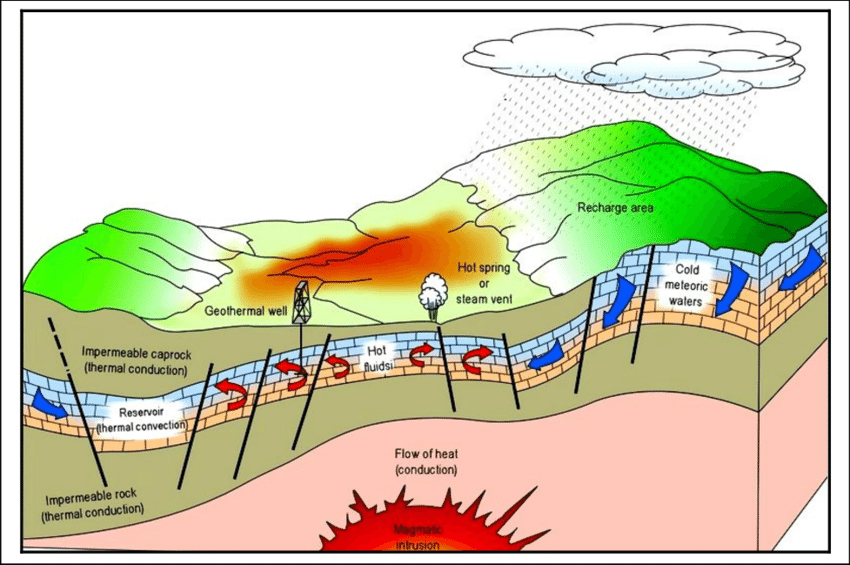
\includegraphics[scale=0.35]{Figs/geothermal.png}
	\caption{Sistem panas bumi}
	\label{fig:geothermal}
\end{figure}

\hspace{25pt}Sistem panas bumi ini mengalami perpindahan panas baik konduksi maupun konveksi. Konduksi terjadi ketika panas dari sumber panas menuju batuan dasar dan konveksi pada fluida yang terperangkap pada zona reservoir. Fluida tersebut akan mengalami kenaikan temperatur dan tekanan sehingga berusaha untuk mencari celah berupa rekahan atau patahan. Fluida yang berhasil mencapai permukaan dapat berupa manifestasi panas bumi seperti hot spring dan fumarol \citep{White1973}. Ilustrasi sistem panas bumi ditunjukkan pada Gambar \ref{fig:geothermal}.

\section{Metode Penginderaan Jauh}
\subsection{Landsat 8}
\hspace{25pt}Landsat adalah suatu program untuk pencitraan permukaan bumi yang dilakukan atas kerjasama \textit{National Aeronautics and Space Administration} (NASA) dan \textit{U.S. Geological Survey} (USGS). Landsat menyediakan data yang berguna untuk penelitian penggunaan lahan atau perubahan lahan dan berbagai bidang lainnya seperti kehutanan, pertanian, geologi, perencanaan wilayah dan pendidikan \citep{USGS2022}. 

\hspace{25pt}Peluncuran satelit pertama dilakukan pada tanggal 23 Juli 1972 yaitu satelit \textit{Earth Resources Technology Satellite} (ERTS-1), yang kemudian berganti nama menjadi Landsat 1. Peluncuran Landsat 2, Landsat 3, dan Landsat 4 menyusul pada tahun 1975, 1978, dan 1982. Ketika Landsat 5 diluncurkan pada tahun 1984, program ini telah memberikan data global berkualitas tinggi dari permukaan bumi selama 28 tahun dan 10 bulan yang secara resmi mencatatkan Rekor Dunia \textit{Guinness} untuk satelit pengamatan bumi yang beroperasi paling lama. Landsat 6 gagal mencapai orbit pada tahun 1993. Landsat 7 berhasil diluncurkan pada tahun 1999. Pada bulan April 2022, Landsat 7 menurunkan orbitnya sejauh 8 kilometer, namun akan terus menyediakan data hingga September 2022. Landsat 8, diluncurkan pada tahun 2013, dan Landsat 9, diluncurkan pada tahun 2021 \citep{USGS2022}.

\begin{table}[h]
	\centering
	\caption{Band 1-11 pada Landsat 8-9 OLI/TIRS beserta panjang geolombang, resolusi dan kegunaannya}
	\adjustbox{max width=\textwidth}{%
	\begin{tabular}{lcccl}
		\hline
		\multicolumn{2}{c}{Nama Band}                                                             & \begin{tabular}[c]{@{}c@{}}Panjang Gelombang\\      $(\mu m)$\end{tabular} & Resolusi (m) & \multicolumn{1}{c}{Kegunaan}                                                                                                                                    \\ \hline
		Coastal/Aerosol                                                                 & Band 1  & 0.43–0.45                                                                     & 30           & \begin{tabular}[c]{@{}l@{}}Pengamatan wilayah pesisir dan   perairan dangkal; \\      studi deteksi aerosol, debu, dan asap.\end{tabular}                       \\
		Blue (B)                                                                        & Band 2  & 0.45–0.51                                                                     & 30           & \begin{tabular}[c]{@{}l@{}}Pemetaan batimetri; pembedaan   tanah/vegetasi, \\      pemetaan tipe hutan, dan identifikasi fitur buatan manusia.\end{tabular}     \\
		Green (G)                                                                       & Band 3  & 0.53–0.59                                                                     & 30           & Vegetasi puncak; penilaian kekuatan tanaman.                                                                                                                    \\
		Red (R)                                                                         & Band 4  & 0.64–0.67                                                                     & 30           & Identifikasi jenis vegetasi; tanah dan fitur perkotaan.                                                                                                         \\
		Near-Infrared (NIR)                                                             & Band 5  & 0.85–0.88                                                                     & 30           & \begin{tabular}[c]{@{}l@{}}Deteksi dan analisis vegetasi;   pemetaan garis pantai \\      dan kandungan biomassa.\end{tabular}                                  \\
		\begin{tabular}[c]{@{}l@{}}Shortwave   Infrared-1 \\      (SWIR-1)\end{tabular} & Band 6  & 1.57–1.65                                                                     & 30           & \begin{tabular}[c]{@{}l@{}}Analisis kadar air/kekeringan   vegetasi; area yang terbakar \\      dan terdampak kebakaran; deteksi kebakaran aktif.\end{tabular}  \\
		\begin{tabular}[c]{@{}l@{}}Shortwave   Infrared-2\\       (SWIR-2)\end{tabular} & Band 7  & 2.11–2.29                                                                     & 30           & \begin{tabular}[c]{@{}l@{}}Deteksi tambahan terhadap titik   api aktif (terutama \\      pada malam hari); analisis kelembaban/kekeringan tanaman.\end{tabular} \\
		Panchromatic (PAN)                                                              & Band 8  & 0.50–0.68                                                                     & 15           & Penajaman citra multispektral ke resolusi yang lebih tinggi.                                                                                                    \\
		Cirrus                                                                          & Band 9  & 1.36–1.38                                                                     & 30           & Deteksi awan cirrus                                                                                                                                             \\
		\multirow{2}{*}{Thermal}                                                        & Band 10 & 10.60–11.19                                                                   & 30           & \multirow{2}{*}{Pemetaan suhu   tanah dan estimasi kelembaban tanah.}                                                                                           \\
		& Band 11 & 11.50–12.51                                                                   & 30           &                                                                                                                                                                 \\ \hline
	\end{tabular}%
}
\label{tab:Landsat}
\end{table}

\hspace{25pt}Satelit Landsat 8 dan Landsat 9 mengorbit Bumi pada ketinggian 705 km dalam petak sepanjang 185km, bergerak dari utara ke selatan di atas sisi Bumi yang disinari matahari dalam orbit sinkron matahari. Setiap satelit melakukan orbit penuh setiap 99 menit, menyelesaikan sekitar 14 orbit penuh setiap hari, dan melintasi setiap titik di Bumi setiap 16 hari sekali. Landsat 8 dan 9 masing-masing memiliki dua sensor yaitu \textit{Operational Land Imager} (OLI) dan \textit{Thermal Infrared Sensor }(TIRS). Satelit ini terdiri dari 11 band dengan rincian 5 band \textit{Visual Near Infrared} (VNIR), 2 band \textit{Short wave Infrared} (SWIR), 1 band \textit{Panchromatic} (PAN), 1 band \textit{cirrus}, dan 2 band \textit{Thermal Infrared} (TIR). Dua band TIR tersebut adalah band 10 dan 11 yang dapat digunakan untuk pemetaan suhu tanah dan estimasi kelembaban tanah. Akan tetapi, karena ketidakpastian kalibrasi yang lebih besar terkait dengan band 11 Landsat 8, disarankan agar tidak menggunakan data band 11 \citep{USGS2022}. Data Landsat 8 dapat diperoleh melalui web \href{https://earthexplorer.usgs.gov/}{https://earthexplorer.usgs.gov/}.Untuk rinician kegunaan dan panjang gelombang masing-masing band dapat dilihat pada tabel \ref{tab:Landsat}

\subsection{\textit{Digital Elevation Model} (DEM)}
\hspace{25pt}\textit{Digital Elevation Model} (DEM) adalah representasi digital dari elevasi permukaan tanah yang berkaitan dengan datum referensi. DEM digunakan untuk menentukan atribut medan seperti elevasi, kemiringan, fitur medan seperti cekungan drainase dan jaringan saluran. DEM digunakan secara luas dalam analisis hidrologi dan geologi, pemantauan bahaya, eksplorasi sumber daya alam, manajemen pertanian, dll.  Beberapa penyedia data DEM adalah DEM SRTM (DEM \textit{Shuttle Radar Topography Mission}) dan DEMNAS (DEM Nasional). 

\hspace{25pt}DEM SRTM 1 Arc Second (30m) adalah data DEM yang disediakan oleh USGS dengan resolusi 30m. Akuisisi dilakukan dengan menerbangkan pesawat ulang-alik Endeavour pada tanggal 11-22 Februari 2000 atas kerja sama \textit{National Aeronautics and Space Administration} (NASA) dan \textit{National Geospatial Intelligence Agency} (NGA). DEM SRTM yang dapat diakses melalui \href{https://earthexplorer.usgs.gov/}{https://earthexplorer.usgs.gov/}\citep{USGSDEM2018}. 

\hspace{25pt}DEMNAS adalah data DEM yang mencakup wilayah Indonesia dan dibangun berdasarkan beberapa sumber data IFSAR (resolusi 5m), TERRASAR-X (resolusi resampling 5m dari resolusi asli 5-10 m) dan ALOS PALSAR (resolusi 11.25 m) serta dengan menambahkan data mass point yang digunakan dalam pembuatan peta Rupabumi Indonesia (RBI). Resolusi spasial DEMNAS adalah 0.27-\textit{arcsecond} dengan menggunakan datum vertikal EGM2008. Sehingga secara resolusi, DEMNAS lebih baik daripada DEM SRTM. DEMNAS dapat diakses melalui \href{https://tanahair.indonesia.go.id/demnas}{https://tanahair.indonesia.go.id/demnas}\citep{DEMNAS}.

\subsection{\textit{Land Surface Temperature}}
Data Landsat 8 dapat digunakan untuk menentukan persebaran panas bumi dilihat dari \textit{Land Surface Temperature }(LST). Diperlukan beberapa tahapan untuk mengolah data Landsat 8 hingga akhirnya diperoleh LST yaitu koreksi radiotermik; \textit{brightness temperature} $(T_B)$; \textit{Normalize Difference Vegetation Index} (NDVI); \textit{proportion of vegetation} $(P_V)$; dan \textit{emissivity} $(\varepsilon)$
\begin{enumerate}
	\item Koreksi Radiotermik\\
	Koreksi ini dilakukan untuk mengonversi nilai masing-masing band yang masih dalam digital number (DN) menjadi top of atmosphere (TOA) spectral radiance (lambda). Tujuannya adalah untuk menghilangkan gangguan atmosfer seperti kabut, asap, dan lainnya \citep{USGS2019}. Persamaannya adalah
	\begin{align}
		L_{\lambda}=M_LQ_{cal}+A_l
	\end{align}
	dengan $L_{\lambda}$ adalah \textit{spectral radiance} $(W/m^{2}\cdot sr\cdot\mu m)$, $M_L$ sebagai faktor skala perkalian pancaran untuk setiap band, $Q_{cal}$ adalah data setiap band yang masih dalam digital number, dan $A_l$ adalah faktor penskalaan ulang aditif band. Besaran-besaran tersebut dapat ditemukan dalam metadata file Landsat dimana nilai $M_L$ diperoleh dari (Reflectance\_Multi\_Band\_x), dan $A_l$ diperoleh dari (Reflectance\_Add\_Band\_x). Koreksi ini dilakukan pada band 4,5, dan 10 \citep{USGS2019}.
	\vskip 5pt
	\item \textit{Brightness Temperature} \\
	\textit{Brightness Temperature} $(T_B)$ untuk suatu permukaan adalah ukuran pancaran radiasi gelombang mikro yang menjalar dari atas atmosfer ke satelit, dapat diperoleh dari fungsi radiasi benda hitam Plank \citep{USGS2019}. Persamaannya adalah
	\begin{align}
		T_B = \frac{K_2}{ln\left ( \frac{K_1}{L_{\lambda}}+1 \right )}
	\end{align}
	dengan $K_1$ dan $K_2$ adalah konstanta konversi termal. Nilai tersebut dapat diperoleh dari metadata (K1\_CONSTANT\_BAND\_10) dan (K2\_CONSTANT\_BAND\_10). Persamaan ini diterapkan untuk band sensor TIRS yaitu band 10 dan 11. Akan tetapi karena band 11 memiliki ketidakpastian yang besar, maka band 11 ini tidak digunakan \citep{AvdanandJovanovska}.
	\vskip 5pt
	\item \textit{Normalize Difference Vegetation Index}\\
	\textit{Normalize Difference Vegetation Index} (NDVI) adalah kapasitas relatif suatu permukaan untuk memancarkan energi dinyatakan sebagai emisivitas spektral permukaan yang ditentukan oleh proporsi energi radiatif benda hitam terhadap energi radiatif permukaan tutupan lahan pada suhu tertentu \citep{Ogunode}. Emisivitas spektral ελ pada panjang gelombang λ untuk berbagai tutupan lahan dapat diestimasi berdasarkan metode ambang batas NDVI (\textit{Normalized Difference Vegetation Index}) yang dikembangkan oleh \citep{SobrinoandJimenezMunoz}. Menurut Menurut metode ini, emisivitas spektral tutupan lahan permukaan permukaan dihitung dengan menggunakan band \textit{Near-Infrared} (band 5) dan \textit{Red }(band 4) dari dari data Landsat 8 untuk menghitung NDVI menurut persamaan berikut
	\begin{align}
		NDVI = \frac{NIR(band\ 5)-R(band\ 4)}{NIR(band\ 5)+R(band\ 4)}
	\end{align}
	Band 4 dan band 5 ini juga perlu koreksi radiotermik seperti pada tahapan pertama agar diperoleh nilai NDVI yang lebih baik. Hal ini juga diperlukan untuk mengoreksi kesalahan akibat pengaruh variasi sudut elevasi matahari dan jarak bumi-matahari \citep{SekertekinArslan}. Algoritma konversi untuk data Landsat-8 OLI, yang diterapkan pada band 4 dan 5, diberikan oleh (USGS, 2019) 
	\begin{align}
		\rho_{\lambda}=\frac{M_{\rho}Q_{cal}+A_{\rho}}{sin(\theta_{SE})}
	\end{align}
	dengan $sin(\theta_{SE})$ adalah sudut elevasi matahari setempat. Sudut elevasi matahari di pusat pemandangan dalam derajat disediakan dalam metadata \textit{sun elevation}.
	\vskip 5pt
	\item \textit{Proportion of Vegetation}\\
	Nilai NDVI di atas diperlukan untuk menghitung proporsi tutupan vegetasi $P_v$ yang merupakan parameter penting untuk menghitung emisivitas permukaan lahan \citep{RouseHass}. Persamaannya adalah
	\begin{align}
		P_v = \left (\frac{NDVI-NDVI_{min}}{NDVI_{max}-NDVI_{min}}  \right )^2
	\end{align}
	dengan $NDVI_{min}$ merupakan nilai respon NDVI pada tanah yang kosong, sedangkan $NDVI_{max}$ sebagai respon parameter NDVI pada area vegetasi yang padat.
	\vskip 5pt	
	\item Emisivitas \\
	Menurut \citep{SobrinoandJimenezMunoz}, nilai emisivitas dapat dihitung dengan mempertimbangkan keragaman tutupan lahan pada area studi, dimana nilai 0,22 ≤ NDVI ≤ 0,87 menunjukkan bahwa piksel-piksel tersebut terdiri dari tanah kosong dan vegetasi. Persamaan emisivitas adalah
	\begin{align}
		\varepsilon = 0.004P_v +0.986
	\end{align}
	\vskip 5pt
	\item \textit{Land Surface Temperature}\\
	Langkah terakhir akan diperoleh nilai \textit{land surface temperature} atau temperatur permukaan lahan dengan menggunakan algoritma \textit{single channel} yang ditunjukkan oleh Persamaan berikut \citep{AvdanandJovanovska}
	\begin{align}
		T_s = \frac{T_B}{1+\left ( \frac{\lambda \kappa_B T_B}{hc} \right )ln\varepsilon}\label{eqn:LST}
	\end{align}
	dengan $\lambda$ adalah panjang gelombang radiasi $(\lambda = 11.5\mu m)$, $\kappa_B$ adalah konstanta Boltzmann $(\kappa_B = 1.38\times 10^{-23}J/K)$, $h$ adalah konstanta Plank $(h = 6.63\times 10^{-34}Js)$ dan $c$ adalah kecepatan cahaya $(c=3\times 10^{8}m/s^2)$. Persamaan \ref{eqn:LST} di atas masih dalam satuan Kelvin. Jika ingin dikonversi kedalam Celcius maka hasil persamaannya
	\begin{align}
		LST(^{\circ}C) = T_s - 273.15(K)
	\end{align}
\end{enumerate}
\subsection{\textit{Fault Fracture Density}}
\hspace{25pt} Keberadaan \textit{hot spring} dan fumarol di suatu daerah mengindikasikan terdapat sumber panas bumi di bawah permukaan. \textit{Hot spring }dan fumarol tersebut adalah manifestasi panas bumi yang terbentuk karena adanya patahan atau sesar (Simmons, 1998).  Sesar dapat diakibatkan oleh aktivitas tektonik atau adanya gaya menekan, menarik atau keduanya pada batuan. Melalui citra satelit, sesar atau bentukan memanjang, batas tepi lainnya yang diasumsikan terbentuk karena proses geologi, akan terlihat seperti garis-garis atau disebut juga kelurusan \textit{(lineament)} sehingga dengan melakukan penarikan kelurusan dapat diketahui kondisi geologi daerah penelitian. Kelurusan dapat diperoleh melalui data DEM yang dikonversikan ke \textit{hillshade }dan kemudian diekstraksi otomatis menggunakan algoritma \textit{LINE}. Proses ini akan menghasilkan peta \textit{fault fracture density} dimana kelurusan dengan densitas yang tinggi berkorelasi dengan ditemukannya manifestasi panas bumi \citep{Noviar}.
\needspace{3\baselineskip}
\section{Metode Gravitasi}
\subsection{Konsep Metode Gravitasi}
\hspace{25pt}Metode gravitasi adalah salah satu metode geofisika yang didasarkan pada variasi nilai pengukuran medan gravitasi yang diakibatkan oleh variasi densitas batuan bawah permukaan. Densitas batuan penyusun kerak bumi tidaklah homogen. Hal ini dapat dipengaruhi oleh berbagai sebab seperti aktivitas tektonik dan vulkanik, kondisi topografi, pasang surut dan dinamika laut. Sehingga dalam pengukuran medan gravitasi dapat dihasilkan data yang cukup berbeda dari daerah disekitaarnya atau disebut anomali gravitasi\citep{Mickus}. 

\hspace{25pt} Pengukuran metode gravitasi menggunakan alat yang disebut gravimeter. Gravimeter dapat mengukur perbedaan medan gravitasi terhadap besaran absolut dan mengukur komponen vertikal medan gravitasi dengan ketelitian hingga 0.01mgal (1 mgal = 0.001 cm/s2) sehingga gravimeter dapat mendeteksi anomali kecil \citep{AmizadehDasgupta}. Prinsip kerja gravimeter didasarkan pada hukum Newton tentang gravitasi. Gaya gravitasi adalah gaya tarik menarik antara dua benda bermassa yang dipisahkan pada jarak tertentu \citep{JacobsRussel}. Persamaan dari gaya gravitasi adalah sebagai berikut.
\begin{align}
	F = G \frac{Mm}{r^{2}} \label{eqn:F1}
\end{align}
dengan G adalah konstanta gravitasi universal ($6.67\times 10^{-11}m^{3}kg^{-1}s^{-2}$), M dan m adalah massa benda (kg), dan r adalah jarak kedua benda (m).
\vskip5pt
%\begin{tabular}{ll}
%F &= Gaya gravitasi (N)\\
%G &= Konstanta gravitasi universal ($6.67\times 10^{-11}m^{3}kg^{-1}s^{-2}$)\\
%M, m &= Massa benda (kg)\\
%r &= Jarak kedua benda (m)\\
%\end{tabular}
%\vskip5pt
\hspace{25pt} Di dalam gravimeter terdapat sistem pegas-massa yang akan mengalami gaya berat. Gaya berat ini terjadi akibat tarik menarik antara sistem pegas-massa dalam gravimeter dengan batuan bawah permukaan sehingga terjadi simpangan dan perubahan panjang pegas \citep{Munadi}. Pada metode gravitasi ini pengukuran yang dilakukan adalah medan gravitasi atau percepatan gravitasi (g). Dengan menggunakan hukum II Newton, maka hubungan gaya gravitasi dan percepatan gravitasi adalah
\begin{align}
	F = mg \label{eqn:F2}
\end{align}
maka dari persamaan \eqref{eqn:F1} dan \eqref{eqn:F2}, dapat diperoleh persamaan percepatan gravitasi
\begin{align}
	g = G \frac{m}{r^{2}} \label{eqn:g}
\end{align}
Pengukuran gravitasi pada permukaan akibat benda anomali $(\Delta m)$ akan memeberikan perubahan gravitasi $\Delta g$. Ilustrasinya ditunjukkan seperti pada gambar \ref{fig:PengukuranGravity}
\begin{figure}[h]
\centering
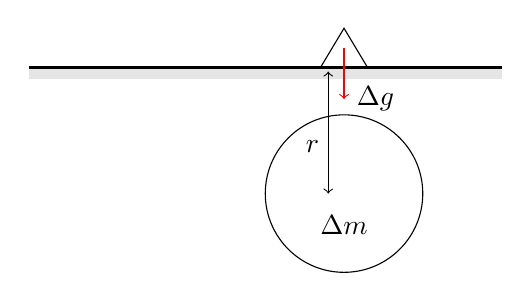
\begin{tikzpicture}
	\filldraw [fill=gray!20, draw=none](0,0)rectangle(6,-0.15);
	\draw [line width=1pt](0,0)--(6,0);
	\draw (4,-1.6) circle (1);
	\draw (3.7,0)--(4,0.5)--(4.3,0)--cycle;
	\draw [<->](3.8,-0.05)--(3.8,-1.6);
	\draw [red, ->](4,0.25)--(4,-0.4);
	\node at (4,-2) {$\Delta m$};
	\node at (3.6,-1){$r$};
	\node at (4.4,-0.4){$\Delta g$};
	
\end{tikzpicture}
\caption{Pengukuran gravitasi di permukaan}
\label{fig:PengukuranGravity}
\end{figure}

Sehingga persamaan \ref{eqn:g} menjadi
\begin{align}
	\Delta g = G \frac{\Delta m}{r^{2}} \label{eqn:g2}
\end{align}

Dimana hubungan massa dengan densitas atau rapat massa adalah $\Delta m = \Delta \rho V $ maka persamaan \ref{eqn:g2} menjadi

\begin{align}
	\Delta g = G \frac{\Delta \rho V}{r^{2}} \label{eqn:g3}
\end{align}

\hspace{25pt}Percepatan gravitasi umumnya memiliki satuan m/s2 atau dalam Gal (dari nama Galileo) yaitu 1cm/s2. Akan tetapi, karena pengukuran percepatan gravitasi dengan selisih yang sangat kecil, maka satuan yang digunakan adalah mGal (miliGal).

\subsection{\textit{Global Gravity Model Plus}(GGMPlus)}
\hspace{25pt} Data gravitasi selain diperoleh dengan pengukuran langsung menggunakan gravimeter, juga dapat diperoleh menggunakan satelit. 	Beberapa penyedia data gravitasi diantaranya adalah \textit{Bureau Gravimetrique International }(BGI), \textit{Global Gravity Model plus }(GGMplus) dan TOPEX. GGMplus adalah model gravitasi hasil inisatif dari Curtin University dan Technical University of Munich yang berbasis pada data satelit GRACE, GOCE, dan EGM2008. Terdapat beberapa data yang disediakan oleh GGMplus yaitu (i) gravity accelerations, (ii) gravity disturbances, (iii) quasigeoid undulations, and (iv) deflection of the vertical components. Keempat jenis data tersebut memiliki resolusi 200 m dan distribusikan dalam grid 5x5 dihitung dengan pemodelan maju gravitasi dari topografi SRTM 7,5 detik busur (\~200 m) dengan mengasumsikan kerapatan konstan 2670 kg m-3.  GGMplus dapat diakses melalui  \href{http://ddfe.curtin.edu.au/gravitymodels/GGMplus/}{http://ddfe.curtin.edu.au/gravitymodels/GGMplus/}\citep{Hirt}
\subsection{Koreksi Gravitasi}
\hspace{25pt} Nilai gravitasi yang diperoleh saat pengukuran di lapangan bukanlah nilai sebenarnya. Nilai tersebut merefleksikan medan gravitasi yang disebabkan oleh semua massa di bumi dan efek rotasi sehingga perlu dilakukannya koreksi \citep{Mariita}. Pengolahan data gravitasi menggunakan data \textit{gravity disturbances (gd)} dari GGMplus telah melalui beberapa tahapan koreksi yaitu koreksi pembacaan alat, tidal, \textit{drift} dan lintang. Sehingga koreksi yang perlu dilakukan adalah koreksi udara bebas \textit{(free air correction)}, koreksi medan \textit{(terrain correction)}, \textit{Bouguer correction} dan terakhir akan diperoleh \textit{Complete Bouguer Anomaly}.

%\begin{enumerate}[label=\alph*)]
\begin{enumerate}
	\item \textit{Free Air Correction}\\
	\textit{Free air correction} atau koreksi udara bebas adalah koreksi nilai gravitasi akibat perbedaan ketinggian titik pengukuran dari permukaan laut (mean sea level) dengan mengabaikan massa diataranya. Koreksi ini perlu dilakukan karena nilai gravitasi teoritis dan observasi harus berada di mean sea level. Pengukuran yang dilakukan pada ketinggian yang berbeda akan menghasilkan nilai gravitasi yang berbeda. Semakin jauh dari pusat bumi nilainya akan berkurang. Perbedaan ketinggian ini memengaruhi nilai gravitasi sebesar 0.3086 mGal/m untuk daerah ekuator hingga lintang 45 atau -45. Nilai ini diperoleh dari persamaan \ref{eqn:gFC} \citep{SleepFujita}
	\begin{align}
		\Delta g_{F}=\frac{2g_{0}h}{R} = 0.3086h\label{eqn:gFC}
	\end{align}
	dengan $g_{0}$ adalah gravitasi absolut (981785 mGal), R adalah jari-jari bumi (6371000 m), dan h adalah ketinggian (m). Sehingga besarnya \textit{free air anomaly} (FAA) pada ketinggian tersebut adalah 
	%\begin{tabular}{ll}
	%	$g_{0}$ &= Gravitasi absolut (981785 mGal)\\
	%	R &= Jari-jari bumi (6371000 m)\\
	%	h &= Ketinggian (m)\\
	%\end{tabular}
	%\vskip 5pt
	\begin{align}
		g_{FAA}=g_{obs}-g(\phi)+0.3086h
	\end{align}
	dengan $g_{obs}$ adalah gravitasi observasi (mGal) dan $g_(\phi)$ adalah gravitasi teroreksi lintang. Untuk pengolahan menggunakan data dari GGMplus persamaannya menjadi
	%\begin{tabular}{ll}
	%	$g_{obs}$ &= Gravitasi observasi (mGal)\\
	%	$g_(\phi)$ &= Gravitasi teroreksi lintang\\
	%	h &= Ketinggian (m)\\
	%\end{tabular}
	%\vskip 5pt
	\begin{align}
		g_{FAA}=g_{d}+0.3086h
	\end{align}
	dengan $g_{d}$ adalah \textit{gravity disturbances} (mGal). Ilustrasi dari pengukuran \textit{free air correction} ditunjukkan pada Gambar \ref{fig:FAC}
	%\begin{tabular}{ll}
	%	$g_{d}$ &= \textit{Gravity disturbances} (mGal)\\
	%	h &= Ketinggian (m)\\
	%\end{tabular}
	%\vskip 5pt
	\begin{figure}[h]
		\centering
		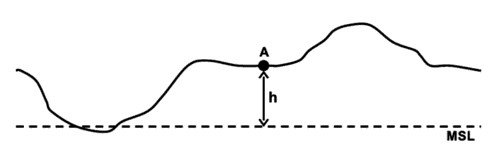
\includegraphics[scale=0.6]{Figs/FAC.jpg}
		\caption{Pengukuran pada ketinggian tertentu terhadap \textit{mean sea level}}
		\label{fig:FAC}
	\end{figure}
	\item \textit{Terrain Correction}\\
	\textit{Terrain Correction} atau koreksi medan dilakukan karena kondisi topografi disekitar titik pengamatan yang tidak beraturan seperti adanya bukit atau lembah. Bukit di titik pengukuran akan menaikkan nilai gravitasi dan sebaliknya jika ada lembah maka akan menurunkan nilai gravitasi \cite{Telford}. Ilustrasinya seperti pada gambar \ref{fig:terrain}
		\begin{figure}
		\centering
		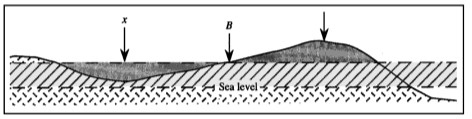
\includegraphics[scale=0.8]{Figs/TC.jpg}
		\caption{Koreksi medan akibat kondisi topografi}
		\label{fig:terrain}
	\end{figure}
	Perhitungan koreksi medan dapat dilakukan menggunakan \textit{hammer chart}. Persamaan dari koreksi medan adalah
	\begin{align}
		\Delta g_{T} (r,\theta)= G\rho\theta\left \{ (r_{0}-r_{i})+\sqrt{r_{i}^{2}+\Delta z^{2}}-\sqrt{r_{0}^{2}+\Delta z^{2}} \right \}
	\end{align}
	dengan $\theta$ adalah sudut pembagian \textit{hammer chart}, $r_{0}$ adalah radius bagian luar suatu zona, $r_{i}$ adalah radius bagian dalam suatu zona, $\Delta z$ adalah perbedaan ketinggian di titik pengamatan $z_{s}$ dengan rata-rata di pembagian zona tersebut $z_{a}$ $(\Delta z = \left | z_{s}-z_{a} \right |)$. Koreksi medan juga dapat dilakukan dengan program komputer menggunakan data \textit{Digital Elevation Model} (DEM).
	%\begin{tabular}{ll}
	%	$\theta$ &= Sudut pembagian \textit{hammer chart}\\
	%	$r_{0}$ &= Radius bagian luar suatu zona\\
	%	$r_{i}$ &= Radius bagian dalam suatu zona\\
	%	$\Delta z$ &= Perbedaan ketinggian di titik pengamatan $z_{s}$ \\ & \hspace{12pt} dengan rata-rata di pembagian zona tersebut $z_{a}$ $(\Delta z = \left | z_{s}-z_{a} \right |)$
	%\end{tabular}
	\vskip 5pt
	\item \textit{Bouguer Correction}\\
	Bouguer Correction atau koreksi Bouguer dilakukan untuk memperhitungkan pengaruh massa yang berada di antara titik pengukuran dan \textit{mean sea level} atau datum. Bouguer adalah nama dari seseorang berkebangsaan Perancis yang melakukan pengamatan di pegunungan Andes, Peru pada tahun 1749. Beliau menyadari bahwa hasil pengukuran dipengaruhi ketinggian dan densitas batuan. Koreksi Bouguer akan mengurangi nilai pengukuran yang dilakukan di atas \textit{mean sea level} dan menambah jika dilakukan di bawah mean sea level. Koreksi ini dilakukan dengan menganggap massa di antara titik pengamatan dan datum sebagai massa silinder berjari-jari tak hingga dengan ketebalan sama dan jarak vertikal titik pengamatan, datum dan densitas disekitar titik pengamatan adalah konstan. Ilustrasinya ditunjukkan seperti pada gambar \ref{fig:BC}. Persamaan dari koreksi Bouguer adalah
	\begin{align}
		\Delta g_{B} = 2\pi G\rho h = 0.04193\rho h\label{eqn:gB}
	\end{align}
	dengan $\rho$ adalah densitas batuan $(g/m^{3})$, dan $h$ adalah ketinggian dari permukaan laut (m).
	\vskip 5pt
	%\begin{tabular}{ll}
	%	$\rho$ &= Densitas batuan $(g/m^{3})$\\
	%	$h$ &= Ketinggian dari permukaan laut (m)
	%\end{tabular}
	\begin{figure}[h]
		\centering
		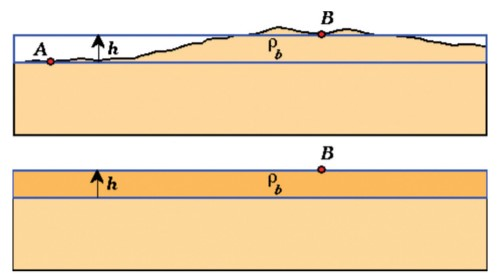
\includegraphics[scale=0.6]{Figs/BC.jpg}
		\captionsetup{justification=centering}
		\caption{Koreksi Bouguer dianggap sebagai massa silinder \\ diantara titik pengukuran dan datum}
		\label{fig:BC}
	\end{figure}
	\item \textit{Complete Bouguer Anomaly}\\
	\textit{Complete Bouguer Anomaly} (CBA) atau anomali Bouguer lengkap dilakukan setelah data pengukuran melalui koreksi-koreksi yang telah disebutkan sebelumnya \citep{Telford}. Maka persamaan dari CBA adalah
	\begin{align}
		g_{CBA} = g_{d} + \Delta g_{F} - \Delta g_{B} + \Delta g_{T}\\
		g_{CBA} = g_{FAA} - \Delta g_{B} + \Delta g_{T} \label{eqn:CBA2}
	\end{align}
	dengan $g_{d}$ adalah \textit{gravity disturbances}, $\Delta g_{F}$ adalah \textit{free air correction}, $\Delta g_{B}$ adalah \textit{Bouguer correction}, $\Delta g_{T}$ adalah \textit{terrain correction}, dan $g_{FAA}$ adalah \textit{free air anomaly}.
	\vskip 5pt
	%\begin{tabular}{ll}
	%	$g_{d}$ &= \textit{Gravity disturbances}\\
	%	$\Delta g_{F}$ &= \textit{Free air correction}\\
	%	$\Delta g_{B}$ &= \textit{Bouguer correction}\\
	%	$\Delta g_{T}$ &= \textit{Terrain correction}\\
	%\end{tabular}
\end{enumerate}
\subsection{Pemisahan Anomali}
\hspace{25pt}\textit{Complete Bouguer Anomaly} yang telah diperoleh merupakan gabungan dari anomali regional, residual (lokal) dan \textit{noise}. Secara kedalaman, anomali regional adalah anomali yang lebih dalam daripada anomali residual dan \textit{noise}. Anomali residual adalah anomali dengan kedalaman lebih dangkal dari regional dan noise sedankan noise lebih dangkal dari anomali residual. Anomali regional diakibatkan oleh anomali dalam dengan frekuensi rendah dan panjang gelombang yang panjang sedangkan anomali residual diakibatkan oleh anomali dangkal dengan frekuensi tinggi dan panjang gelombang yang pendek. Eksplorasi menggunakan metode gravitasi memerlukan informasi mengenai struktur bawah permukaan yang dapat diperoleh dari anomali residual \citep{Telford}. Maka dari itu CBA perlu dilakukan pemisahan anomali sehingga diperoleh anomali residualnya saja. Pemisahan anomali residual dapat dilakukan menggunakan \textit{Butterworth filter}. \textit{Butterworth filter} adalah filter high-pass frekuensi yang digunakan untuk meningkatkan panjang gelombang anomali yang terkait dengan sumber dangkal.
\subsection{Analisa Derivatif}
\hspace{25pt} Anomali residual yang telah diperoleh sudah dapat digunakan untuk interpretasi struktur geologi. Akan tetapi dapat dilakukan proses lanjutan yaitu analisis derivatif seperti \textit{First Horizontal Derivative }(FHD) dan \textit{Second Vertical Derivative}(SVD). FHD dilakukan untuk mengetahui kemenerusan suatu anomali bawah permukaan berdasarkan turunan pertama secara horizontal (Reynold, 1997). Persamaan dari FHD adalah
\begin{align}
	FHD = \sqrt{\left ( \frac{\partial g}{\partial x} \right )^{2}+\left ( \frac{\partial g}{\partial y} \right )^{2}}
\end{align}
SVD dilakukan untuk memperjelas anomali residual sehingga struktur seperti sesar atau patahan dapat terlihat lebih jelas. Penentuan jenis sesar baik naik, turun ataupun geser dapat ditentukan dari nilai maksimum dan minimum turunan kedua nilai gravitasi terhadap arah vertikal \citep{Sarkowi}
\begin{itemize}
	\item Nilai $\left | \frac{\partial^2g}{\partial z^2} \right |_{max} > \left | \frac{\partial^2g}{\partial z^2} \right |_{min}$ mengindikasikan sesar turun 
	\item Nilai $\left | \frac{\partial^2g}{\partial z^2} \right |_{max} < \left | \frac{\partial^2g}{\partial z^2} \right |_{min}$ mengindikasikan sesar naik
	\item Nilai $\left | \frac{\partial^2g}{\partial z^2} \right |_{max} = \left | \frac{\partial^2g}{\partial z^2} \right |_{min}$ mengindikasikan sesar geser
\end{itemize}
\section{Densitas Batuan}
\hspace{25pt} Densitas batuan merupakan besaran yang menentukan nilai percepatan gravitasi. Beberapa hal yang dapat memengaruhi nilai densitas batuan yaitu kerapatan butir pembentuknya, porositas, kandungan fluida yang mengisi pori, dan pemadatan akibat tekanan dan pelapukan \citep{Kirbani}. Nilai densitas beberapa batuan ditunjukkan pada tabel \ref{tab:density}.
\begin{table}[h]
	\centering
	\caption{Densitas beberapa jenis batuan (Telford,1990)}
	\label{tab:density}
	\adjustbox{scale=0.7}{%
	\begin{tabular}{ccc}
		\hline
		Jenis Batuan   & \begin{tabular}[c]{@{}c@{}}Rentang Densitas\\ (g/cm3)\end{tabular} & \begin{tabular}[c]{@{}c@{}}Densitas Rata-Rata\\ (g/cm3)\end{tabular} \\ \hline
		\multicolumn{3}{c}{Batuan Sedimen}                                                                                                                         \\ \hline
		Overburden     &                                                                    & 1.92                                                                 \\
		Soil           & 1.20 - 2.40                                                        & 1.92                                                                 \\
		Clay           & 1.63 - 2.60                                                        & 2.21                                                                 \\
		Gravel         & 1.70 - 2.40                                                        & 2.00                                                                 \\
		Sand           & 1.70 - 2.30                                                        & 2.00                                                                 \\
		Sandstone      & 1.61 - 2.76                                                        & 2.35                                                                 \\
		Shale          & 1.77 - 3.20                                                        & 2.40                                                                 \\
		Limestone      & 1.93 - 2.90                                                        & 2.55                                                                 \\
		Dolomite       & 2.28 - 2.90                                                        & 2.70                                                                 \\ \hline
		\multicolumn{3}{c}{Batuan Beku}                                                                                                                            \\ \hline
		Rhyolite       & 2.35 - 2.70                                                        & 2.52                                                                 \\
		Andesite       & 2.40 - 2.80                                                        & 2.61                                                                 \\
		Granite        & 2.50 - 2.81                                                        & 2.64                                                                 \\
		Granodiorite   & 2.67 - 2.79                                                        & 2.73                                                                 \\
		Porphyry       & 2.60 - 2.89                                                        & 2.74                                                                 \\
		Quartz diorite & 2.62 - 2.96                                                        & 2.79                                                                 \\
		Diorite        & 2.72 - 2.99                                                        & 2.85                                                                 \\
		Lavas          & 2.80 - 3.00                                                        & 2.90                                                                 \\
		Diabase        & 2.50 - 3.20                                                        & 2.91                                                                 \\
		Basalt         & 2.70 - 3.30                                                        & 2.99                                                                 \\
		Gabbro         & 2.70 - 3.50                                                        & 3.03                                                                 \\
		Periodotite    & 2.78 - 3.37                                                        & 3.15                                                                 \\
		Acid igneous   & 2.30 - 3.11                                                        & 2.61                                                                 \\
		Basic igneous  & 2.09 - 3.17                                                        & 2.79                                                                 \\ \hline
		\multicolumn{3}{c}{Batuan Metamorf}                                                                                                                        \\ \hline
		Quarzite       & 2.50 - 2.70                                                        & 2.60                                                                 \\
		Schists        & 2.39 - 2.90                                                        & 2.64                                                                 \\
		Graywacke      & 2.60 - 2.70                                                        & 2.65                                                                 \\
		Marble         & 2.60 - 2.90                                                        & 2.75                                                                 \\
		Serpentine     & 2.40 - 3.10                                                        & 2.78                                                                 \\
		Slate          & 2.70 - 2.90                                                        & 2.79                                                                 \\
		Gneiss         & 2.59 - 3.00                                                        & 2.80                                                                 \\
		Amphibolite    & 2.90 - 3.04                                                        & 2.96                                                                 \\
		Eclogite       & 3.20 - 3.54                                                        & 3.37                                                                 \\
		Metamorpic     & 2.40 - 3.10                                                        & 2.74                                                                 \\ \hline
	\end{tabular}%
}
\end{table}
Penentuan densitas rata-rata bawah permukaan atau densitas Bouguer dapat dihitung menggunakan metode Parasnis. Metode ini menggunakan pendekatan analitis dengan mengasumsikan tidak ada korelasi antara topografi dengan densitas permukaan sehingga anomali tersebar secara acak. Maka \textit{Complete Bouguer Anomaly} dapat dianggap nol  sehingga dari persamaan \ref{eqn:CBA2} diperoleh
\begin{align}
g_{FAA}-\Delta g_{B}+\Delta g_{T}&=0\\
g_{FAA}-0.04193\rho h+\Delta g_{T}&=0\\
g_{FAA}&=0.04193\rho h-\Delta g_{T}\\
g_{FAA}&=\rho \left (0.04193 h-\frac{\Delta g_{T}}{\rho_0}  \right )\label{eqn:Parasnis}
\end{align}
dengan $\rho_0$ adalah densitas rata-rata dipermukaan bumi yaitu $2.67 g/cm^2$.  Kemudian dilakukan regresi linier dimana sumbu x adalah $\left (0.04193 h-\frac{\Delta g_{T}}{\rho_0}  \right )$ dan sumbu y adalah $g_{FAA}$ sehingga akan diperoleh nilai $\rho$ \citep{Telford}.
